\documentclass{beamer}

% Theme choice
\usetheme{CambridgeUS} % professional, clean look
\usecolortheme{default} % colors can be adjusted if desired

% Packages
\usepackage[utf8]{inputenc}
\usepackage{graphicx}   % for including graphics
\usepackage{booktabs}   % for tables
\usepackage{amsmath, amssymb} % for math
\usepackage{hyperref}   % for clickable links

% Title page info
\title[]{Presentation of 'Employer Consolidation and Wages: Evidence from the Hospital Industry'}
\subtitle{Written by: Elena Prager and Matt Schmitt}
\author[Your Name]{Tate Mason\\ \smallskip \texttt{Tate.Mason@uga.edu}}
\date{\today} % or custom date

% Begin document
\begin{document}

% Title page
\begin{frame}
  \titlepage
\end{frame}

% Outline
\begin{frame}{Outline}
  \tableofcontents
\end{frame}

% Section 1
\section{Introduction}

\begin{frame}{Research Question}
  \begin{block}{Main Question}
    What is the effect of hospital mergers on the wages of hospital workers?
  \end{block}
  \pause
  \begin{exampleblock}{Key Findings}
    The authors find that hospital mergers lead to decreases in wages for certain categories of hospital workers, particularly nurses and technicians.
  \end{exampleblock}
\end{frame}

% Section 2
\section{Methodology}

\begin{frame}{Data}
  \begin{itemize}
    \item Datasets:
    \begin{itemize}
      \item CMS Health Care Cost Report Information System (HCRIS)
      \item BLS Current Population Survey (CPS) and Quarterly Census of Employment and Wages (QCEW)
      \item American Hospital Association (AHA) Annual Survey
      \item Mergers and Acquisitions data from Irving Levin Associates
      \item Census data for commuting zones
    \end{itemize}
    \item Sample Period: 2000 - 2010 
  \end{itemize}
\end{frame}

\begin{frame}{HCRIS and AHA Annual Survey}
  \begin{itemize}
    \item HCRIS:
    \begin{itemize}
      \item Provides hospital-level financial and operational data
      \item Key variables: number of employees by occupation, wages, hospital characteristics
    \end{itemize}
    \item AHA: Provides detailed information on hospital characteristics, services, and ownership
  \end{itemize}
\end{frame}

\begin{frame}{CPS and QCEW}
  \begin{itemize}
    \item CPS: Individual-level data on employment, wages, demographics
    \item QCEW: Establishment-level data on employment and wages by industry
  \end{itemize}
\end{frame}

\begin{frame}{Mergers and Acquisitions Data and Commuting Zones}
  \begin{itemize}
    \item Mergers data from Irving Levin Associates
    \begin{itemize}
      \item Data on hospital mergers from Irving Levin Associates
      \item Key variables: merger date, involved hospitals, market definitions
    \end{itemize}
    \item Commuting Zones (CZ)
    \begin{itemize}
      \item Used to define local labor markets
      \item Based on commuting patterns from Census data
    \end{itemize}
  \end{itemize}
\end{frame}

\begin{frame}{Empirical Strategy}
  \begin{itemize}
    \item Difference-in-Differences (DiD) approach
    \item Commuting zones whcih experienced a single merger-induced concentration increase
    \begin{itemize}
      \item Treatment group: CZs with a hospital merger (84 CZ)
      \item Control group: CZs without a hospital merger (293 CZ)
    \end{itemize}
  \end{itemize}
\end{frame}

\begin{frame}{Summary Statistics}
summar
\end{frame}

\begin{frame}{Model}
  \begin{equation}
    ln(wage_{imt}) = \delta_i + \tau_t + \alpha post_{mt} + X_{imt}\beta + \epsilon_{imt}
  \end{equation}
\end{frame}

\begin{frame}{Identification}
  \begin{itemize}
    \item Parallel trends assumption
    \item Control for time-invariant differences across CZs and common time shocks
    \item Robustness checks: varying control groups, alternative specifications
  \end{itemize}
\end{frame}

\begin{frame}{Parallel Trends Check}
  \begin{figure}
    \centering
    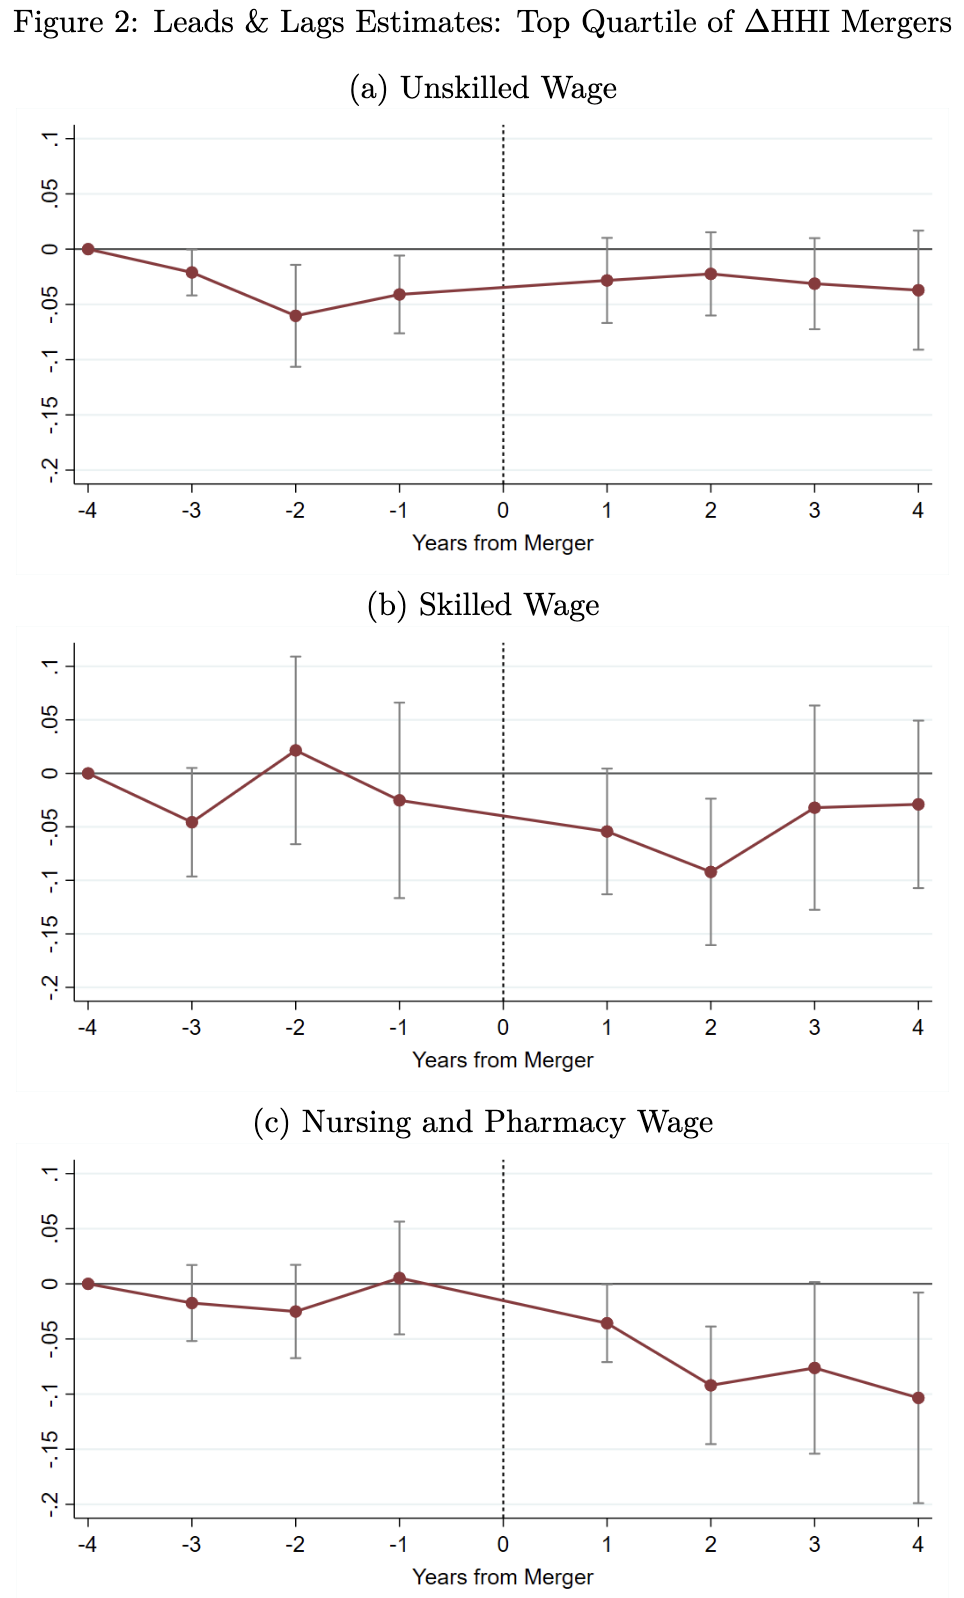
\includegraphics[width=0.33\textwidth]{parallel_trends.png}
    \caption{Wage trend differences (top quartile of mergers)}
  \end{figure}
\end{frame}

% Section 3
\section{Results}

\begin{frame}{Main Results}
  \begin{figure}
    \centering
    \caption{Main empirical finding}
  \end{figure}
\end{frame}

\begin{frame}{Table of Results}
  \begin{table}
    \centering
    \begin{tabular}{lcc}
      \toprule
      Variable & Coef. & Std. Error \\
      \midrule
      $X$ & 0.45 & 0.12 \\
      $Z$ & -0.23 & 0.08 \\
      \bottomrule
    \end{tabular}
    \caption{Regression results}
  \end{table}
\end{frame}

% Section 4
\section{Conclusion}

\begin{frame}{Conclusion}
  \begin{itemize}
    \item Summarize findings
    \item Contributions
    \item Future work
  \end{itemize}
\end{frame}

\end{document}
